\section{Aims}
\paragraph{} At the end of the practical portion of this topic you will be able to:

\begin{itemize}
\item Retrieve data from Web Service APIs using JSON
\item Use Google Services
\end{itemize}

\section{Web Service APIs \& JSON}
\paragraph{} In this part of the practical we are going to retrieve some data in the JSON format from a web API, i.e. a location on the web with an address that starts with HTTP or HTTPS. JSON is a simple format for describing data. There is a useful online editor for writing and testing JSON documents at JSONLint\footnote{\url{http://jsonlint.com/}} and the JSON syntax is described on the JSON.org website\footnote{\url{http://json.org/}}. This is an example JSON document, retrieved from the geoip JSON feed \footnote{\url{http://www.telize.com/geoip}}:

\begin{lstlisting}
{"longitude":-0.13,"latitude":51.5,"asn":"AS2529","offset":"1","ip":"80.176.131.121","area_code":"0","continent_code":"EU","dma_code":"0","timezone":"Europe\/London","country_code":"GB","isp":"Now maintained by Cable ","country":"United Kingdom","country_code3":"GBR"}
\end{lstlisting}

\paragraph{} For our example Android app we will create a layout that has a TextView (to relay messages to us) and a multiline EditText (to display the contents of the retrieved JSON document). In addition we will need to add some permissions to the Android manifest and we need a new inner classe and some extrac methods in our MainActivity class. So, lets get started. Add the following permissions to AndroidManifest.xml:

\begin{lstlisting}
    <uses-permission android:name="android.permission.INTERNET"/>
    <uses-permission android:name="android.permission.ACCESS_NETWORK_STATE"/>
\end{lstlisting}
       
\paragraph{} Now we need to add a string to strings.xml for use by our TextView

\begin{lstlisting}
    <string name="status_msg">Connected?</string>
\end{lstlisting}

\paragraph{} We can now assemble our layout in activity\_main.xml by deleting the `hello world' TextView and adding the following as children of the default RelativeLayout:

\begin{lstlisting}
<LinearLayout
        android:orientation="vertical"
        android:layout_width="fill_parent"
        android:layout_height="fill_parent"
        android:layout_alignParentTop="true"
        android:layout_alignParentRight="true"
        android:layout_alignParentEnd="true">

        <TextView
            android:layout_width="fill_parent"
            android:layout_height="wrap_content"
            android:text="@string/status_msg"
            android:id="@+id/tv1" />

        <EditText
            android:layout_width="match_parent"
            android:layout_height="fill_parent"
            android:id="@+id/et1"
            android:ems="10"
            android:inputType="textMultiLine"
            android:layout_gravity="center_horizontal" />
    </LinearLayout>
\end{lstlisting}

\paragraph{} Now we can edit MainActivity.java to actually do something. First we need some variables in the MainActivity class:

\begin{lstlisting}
    EditText etResponse;
    TextView tvConnected;
\end{lstlisting}

\paragraph{} Now we can add the following three methods to the MainActivity class:

\begin{lstlisting}
public static String GET(String url)
    {
        InputStream inStream = null;
        String result = "";
        try
        {
            HttpClient httpClient = new DefaultHttpClient();
            HttpResponse httpResponse = httpClient.execute(new HttpGet(url));
            inStream = httpResponse.getEntity().getContent();
            if(inStream != null)
                result = convertInputStreamToString(inStream);
            else
                result = "Did not work";
        }
        catch (Exception e)
        {
            Log.d("InputStream", e.getLocalizedMessage());
        }
        return result;
    }

    private static String convertInputStreamToString(InputStream inputStream) throws IOException
    {
        BufferedReader br = new BufferedReader( new InputStreamReader(inputStream));
        String line = "";
        String result = "";
        while((line = br.readLine()) != null )
            result += line;
        inputStream.close();
        return result;
    }

    public boolean  isConnected()
    {
        ConnectivityManager cman = (ConnectivityManager) getSystemService(Activity.CONNECTIVITY_SERVICE);
        NetworkInfo netinfo = cman.getActiveNetworkInfo();
        if(netinfo != null && netinfo.isConnected())
            return true;
        else
            return false;
    }
\end{lstlisting}

\paragraph{} These give us a couple of utility methods to check whether we are connected to the web (isConnected), convert an InputStream into a String (convertInputStreamToString) and the important method (GET) that performs our important HTTP GET action which actually does the job of connecting to the remote web-service and retrieving a JSON document. Next we can implement an inner class within the MainActivity class which will control performing our GET in a separate task so that we don't affect the main app control thread whilst waiting for the remote server to respond and complete the transmission of the data. Because it can take a while for a remote service to respond, for example because the server is heavily loaded, or offline, or because the payload, the document returned, is very large, you should always perform these calls as an asynchronous task that won't directly affect the other important things that your app needs to do, like responding to user input.

\begin{lstlisting}
    private class HttpAsyncTask extends AsyncTask<String, Void, String>
    {
        @Override
        protected String doInBackground(String... urls)
        {
            return GET(urls[0]);
        }
        @Override
        protected void onPostExecute(String result)
        {
            Toast.makeText(getBaseContext(), "Received", Toast.LENGTH_SHORT).show();
            etResponse.setText(result);
        }
    }
\end{lstlisting}

\paragraph{} Now, finally, we can use all of these methods and inner classes to actually do something. Our final bit of code will go into the onCreate method of the MainActivity class:

\begin{lstlisting}
protected void onCreate(Bundle savedInstanceState) {
        super.onCreate(savedInstanceState);
        setContentView(R.layout.activity_main);

        etResponse = (EditText) findViewById(R.id.et1);
        tvConnected = (TextView) findViewById(R.id.tv1);

        if(isConnected())
        {
            tvConnected.setBackgroundColor(0xFF00CC00);
            tvConnected.setText("You are connected");
        }
        else
        {
            tvConnected.setText("Not Connected");
        }
        new HttpAsyncTask().execute("http://jsonip.com");
    }
\end{lstlisting}

\paragraph{} You should now be able to run your app and the response from the url in this line:

\begin{lstlisting}
new HttpAsyncTask().execute("http://jsonip.com");
\end{lstlisting}

\paragraph{} will be displayed. You can also put that url \url{http://jsonip.com} into a web browser to compare what response you get.

\section{Google Play Services}
\subsection{Requirements}
\paragraph{} The following tutorial is easiest to complete if you have your own Android device to debug on.  Google Maps requires that the device have Google API platform installed as well as be able to run OpenGL 2.0, these requirements make it a hassle to try to test on a default virtual device.  Developing a Google Maps app also requires the “Google Play Services” package, this can be installed from the SDK Manager under ‘Extras’.

\begin{figure}[H]%[htb]
\centering
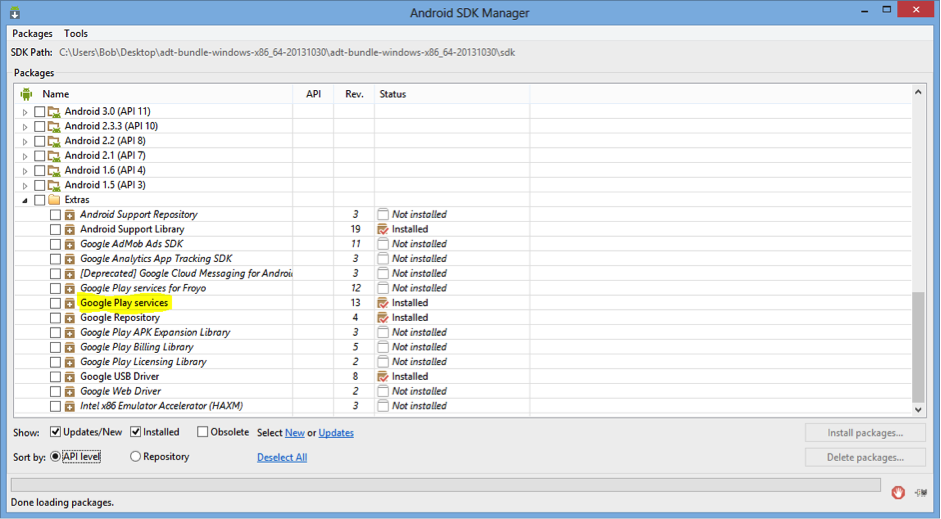
\includegraphics[width=\textwidth]{images/eclipse_sdk-manager}
\caption{SDK manager window of Eclipse showing Google Play Services}
\label{fig:eclipse-sdk-manager}
\end{figure}

\paragraph{} Requirements:

\begin{itemize}
\item Android device
\item Google Account (to get an API key)
\item Google Play Services Package
\end{itemize}

\subsection{Acquiring an API key}
\paragraph{} In order to use Google’s APIs you need an API key.  To get a maps key go to the Google APIs page\footnote{\url{https://code.google.com/apis/console}} and agree to the terms and conditions. You should now be on a page that looks similar to the following, browse down the list of APIs until you find “Google Maps Android API v2” and switch it to ON.

\begin{figure}[H]%[htb]
\centering
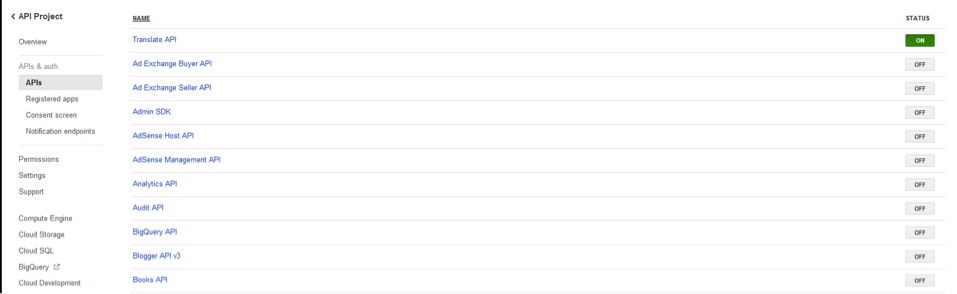
\includegraphics[width=\textwidth]{images/google-maps-api-page}
\caption{Google Maps API page}
\label{fig:google-maps-api-page}
\end{figure}

\paragraph{} Now that it’s on, go to ``Credentials'' on the left side and click the ``CREATE NEW KEY'' button and choose ``Android key''.  In the following text field you will need to provide the package name and SHA1 fingerprint. For package name type in zzcom.example.gmapsexample'' (NOTE: If you named your application something else use that name instead). To get your SHA1 fingerprint go to Window $>$ Preferences $>$ Android $>$ Build in Eclipse and copy the hexadecimal numbers from the SHA1 fingerprint box into the registration page. Once you click register, choose the “Android Key” option and copy the API key for use later.

\subsection{Preparing the Manifest}
\paragraph{} First things first, we need to import the Google Play Services to the workspace, go to File > Import > Existing Android Code Into Workspace.  Now browse to your SDK folder and go to 

\begin{framed}
Extras/google/google\_play\_services
\end{framed}
\paragraph{} Select the ‘libproject’ folder and click ok.

\begin{figure}[H]%[htb]
\centering
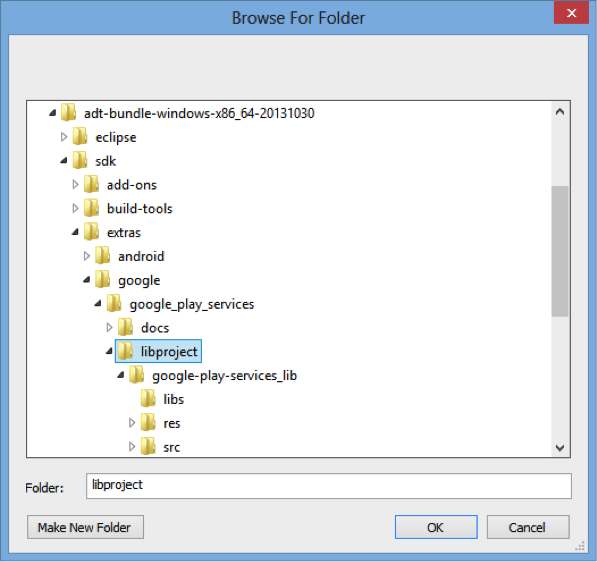
\includegraphics[width=0.75\textwidth]{images/libproject}
\caption{Google Maps API page}
\label{fig:libproject}
\end{figure}

\paragraph{} One project should be listed, check the “Copy projects into workspace” box then click finish. Now new Android Application named ‘GMapsExample’.  Now we need to add Google Play Services as a reference to our application. To do this, right click on your App in the package explorer and go to properties.  From properties go to Android on the left hand side and choose ‘Add…’ in the library section, highlight the “google-play-services\_lib” project and click ok.

\begin{figure}[H]%[htb]
\centering
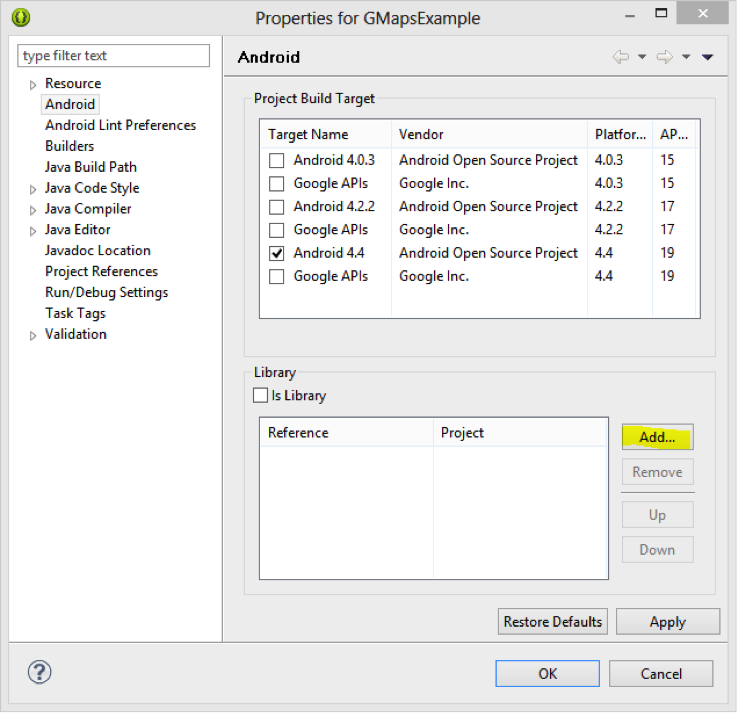
\includegraphics[width=0.75\textwidth]{images/gplay-services-lib}
\caption{Google Play Services Lib}
\label{fig:gplay-services-lib}
\end{figure}

\paragraph{} The final step to referencing play services is to add the following XML to our manifest within the <application> element.

\begin{lstlisting}
<meta-data
    	android:name="com.google.android.gms.version"
    	android:value="@integer/google_play_services_version" />
\end{lstlisting}

\paragraph{} Now that we have referenced the play services, we need to add the following permissions to our manifest to allow the application to get the users location and access Google’s servers.

\begin{lstlisting}
<!-- Used to download tiles from servers -->
<uses-permission android:name="android.permission.INTERNET" />
<!-- Used to check the network state to determine if data can be downloaded -->
<uses-permission android:name="android.permission.ACCESS_NETWORK_STATE" />
<!-- Used to cache map tiles -->
<uses-permission android:name="android.permission.WRITE_EXTERNAL_STORAGE" />
<!-- Allows access to google web services -->
<uses-permission android:name="com.google.android.providers.gsf.permission.READ_GSERVICES"/>
<!-- Allows app to access phones GPS information -->
<uses-permission android:name="android.permission.ACCESS_FINE_LOCATION" />
\end{lstlisting}

\paragraph{} Google Maps uses OpenGL ES v2 to render the map, we need to specify in the apps manifest that our app will be using this feature by adding the following to the manifest (just after the permissions).

\begin{lstlisting}
<uses-feature
        android:glEsVersion="0x00020000"
        android:required="true"/>
\end{lstlisting}

\paragraph{} Lastly we need to add the API key from the last step into our manifest. To do this simply copy the following section and paste it just after the other meta-data tags we added in the <application> element, remembering to replace the android:value value with your own API key.

\begin{lstlisting}
<meta-data android:name="com.google.android.maps.v2.API_KEY"
    		android:value="YOUR KEY HERE"/>
\end{lstlisting}

\subsection{Building the Application}
\paragraph{} Now that's all out the way we can get to building the app, the first step is to add a map fragment to your layout.  Open up your main\_activity layout and replace the XML with the following.

\begin{lstlisting}
<?xml version="1.0" encoding="utf-8"?>
<fragment xmlns:android="http://schemas.android.com/apk/res/android"
          android:id="@+id/map"
          android:layout_width="match_parent"
          android:layout_height="match_parent"
          android:name="com.google.android.gms.maps.MapFragment"/>
\end{lstlisting}

\paragraph{} If you run your app now you should get a screen looking something like this, if not then check your LogCat messages for any indication of what the issue may be. Often it will be an issue with API keys. Ensure the details of your application have been correctly registered on the API console and that you have correctly added your API key to the manifest and try again.

\begin{figure}[H]%[htb]
\centering
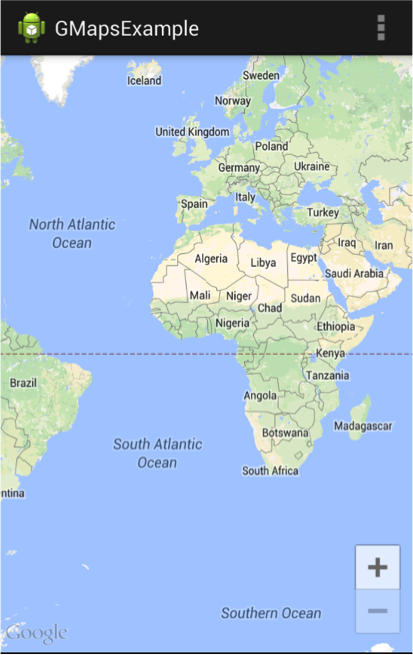
\includegraphics[width=0.5\textwidth]{images/google-map-example}
\caption{Google Map Screen}
\label{fig:google-map-example}
\end{figure}

\paragraph{} Now we’re going to make the map centre on the phones GPS position.  First set up a LocationManager and Listener just like section 4 of Week 3s tutorial, but this time replace the code inside the onLocationChanged function to the following.

\begin{lstlisting}
if (location != null) {
	GoogleMap map = ((MapFragment) getFragmentManager().findFragmentById(R.id.map)).getMap();
					
					map.moveCamera(CameraUpdateFactory.newLatLngZoom(new LatLng(location.getLatitude(), location.getLongitude()), 13));
}
\end{lstlisting}

\paragraph{} The first line here retrieves the map fragment from the layout and stores it in a variable called map (much like findViewById does for buttons and such) while the second line moves the camera by using a CameraUpdateFactory and providing it with a new LatLng object (created using the latitude and longitude values from the location variable) and a zoom level.

\paragraph{Extra Tasks} Try adding some buttons to the application that take you directly to different places.

\subsection{More Features}

\paragraph{} There are several other ways we can interact and modify the maps.  We can choose between the following:

\begin{itemize}
\item Normal – Roads, man-made features and important natural features (eg rivers) shown
\item Hybrid – Satellite picture with roads added
\item Satellite – Satellite picture, no roads added
\item Terrain – Topographic data, includes colours/contour lines
\end{itemize}

\paragraph{} To choose a different map style we simple have to call the setMapType function and tell it which type we want.

\begin{lstlisting}
map.setMapType(GoogleMap.MAP_TYPE_SATELLITE);
/* GoogleMap.MAP_TYPE_NORMAL
 * GoogleMap.MAP_TYPE_HYBRID
 * GoogleMap.MAP_TYPE_TERRAIN
 */
\end{lstlisting}

\paragraph{} The following shows an example of normal, hybrid and terrain maps for the same location.

\begin{figure}[H]%[htb]
\centering
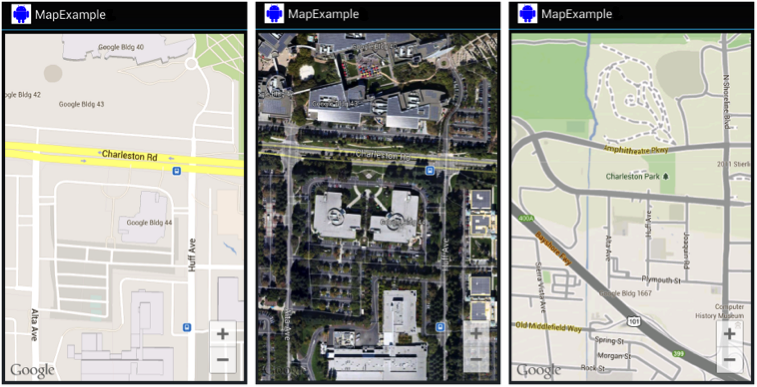
\includegraphics[width=\textwidth]{images/normal-hybrid-terrain-map-examples}
\caption{Examples of Normal, Hyrbid, \& Terrain Google Maps}
\label{fig:normal-hybrid-terrain-map-examples}
\end{figure}

\subsubsection{Markers}
\paragraph{} We can also draw several different things onto the maps such as markers or information windows.  Adding a marker onto Edinburgh Castle is as simple as the following.

\begin{lstlisting}
LatLng edCastle = new LatLng(55.948611, -3.200833);
map.addMarker(new MarkerOptions().position(edCastle));
\end{lstlisting}

\paragraph{} The first line creates a LatLng object with the coordinates of Edinburgh Castle and the second line adds a new marker to the map object at the coordinates of edCastle.  You can add loads of other options to your markers such as making them draggable, changing their colour, using your own image as the marker icon or even adding click or drag events to the markers.  For more information on how to customise your markers see the Marker documentation\footnote{\url{https://developers.google.com/maps/documentation/android/marker\#customize_a_marker}}.

\subsubsection{Information Windows}
\paragraph{} Markers are great for, well, marking a position on the map.  However sometimes we want to display some information at a point on the map.  To do this we can use info windows.  To do this we create a marker on the map much the same as we did before, except this time we give it a title and snippet.  Replace your marker from the last step with the following

\begin{lstlisting}
map.addMarker(new MarkerOptions().position(edCastle).title("Edinburgh Castle").snippet("Historic fortress which dominates the skyline of the city of Edinburgh, Scotland"));
\end{lstlisting}

\paragraph{} Run the application again, you’ll see a marker on Edinburgh Castle much like before except this time when you click it some extra information will be shown

\begin{figure}[H]%[htb]
\centering
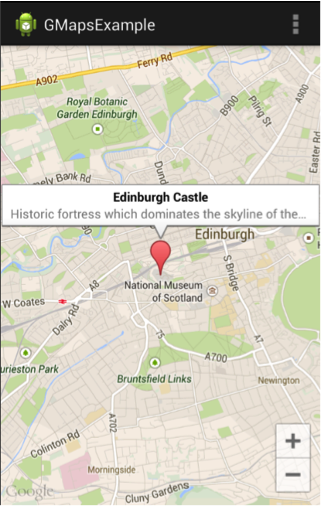
\includegraphics[width=0.5\textwidth]{images/google-map-info-marker}
\caption{Google Map Marker Example}
\label{fig:google-map-info-marker}
\end{figure}


\section{Summary}
\paragraph{} In this practical we have 

\begin{itemize}
\item Retrieve data from Web Service APIs using JSON
\item Use Google Services
\end{itemize}


